\documentclass[tikz,border=8pt]{standalone}
\usepackage{amsmath,amssymb}
\usepackage{tikz}
\usepackage{pgfplots}
\pgfplotsset{compat=1.18}
\begin{document}
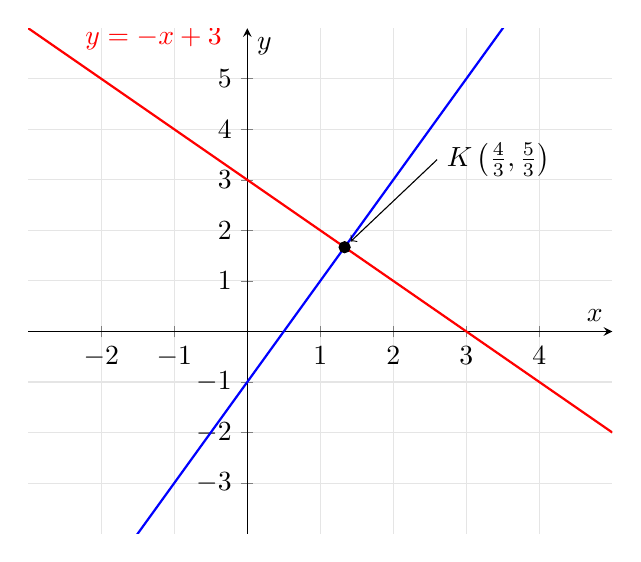
\begin{tikzpicture}
  \begin{axis}[
    axis lines=middle, xlabel={$x$}, ylabel={$y$},
    xmin=-3, xmax=5, ymin=-4, ymax=6,
    xtick={-2,...,4}, ytick={-3,...,5},
    grid=both, grid style={gray!20},
    width=9cm, height=8cm, samples=2,
  ]
    \addplot[thick, blue, domain=-3:5] {2*x - 1} node[pos=0.92, left] {$y=2x-1$};
    \addplot[thick, red,  domain=-3:5] {-x + 3}  node[pos=0.08, above right] {$y=-x+3$};
    \addplot[only marks, mark=*] coordinates {(4/3, 5/3)};
    \draw[<-, shorten <=3pt] (axis cs:4/3,5/3) -- (axis cs:2.6,3.4)
      node[right] {$K\left(\tfrac43,\tfrac53\right)$};
  \end{axis}
\end{tikzpicture}
\end{document}
